\documentclass[12pt, a4paper]{article}

\usepackage[utf8]{inputenc}

% Limit the page margin to only 1 inch.
\usepackage[margin=1in]{geometry}

%Imports biblatex package
\usepackage[
backend=biber,
style=alphabetic
]{biblatex}
\addbibresource{../math-342w.bib}

% Enables the `align' environment.
\usepackage{amsmath}

% Provides useful environments, such as:
% - \begin{proof} ...\end{proof}
\usepackage{amsthm}
\newtheorem{proposition}{Proposition}
\theoremstyle{definition}
\newtheorem*{definition}{Definition}
\newtheorem{theorem}{Theorem}
\newtheorem{corollary}{Corollary}

% Enables using \mathbb{}, for example \mathbb{N} for the set of natural numbers.
\usepackage{amssymb}

% Allows using letters in enumerate list environment. Use, for example:
%\begin{enumerate}[label=(\alph*)]
% ...
%\end{enumerate}
\usepackage[inline]{enumitem}

% Enable importing external graphic files and provides useful commands, like \graphicspath{}
\usepackage{graphicx}
% Images are located in a directory called "images" in the current directory.
\graphicspath{{./images/}}

% Make links look better by default.
% See: https://tex.stackexchange.com/questions/823/remove-ugly-borders-around-clickable-cross-references-and-hyperlinks
\usepackage[hidelinks]{hyperref}
\usepackage{xcolor}
\hypersetup{
	colorlinks,
	linkcolor={red!50!black},
	citecolor={blue!50!black},
	urlcolor={blue!80!black}
}

% Code Listings. Source:
% https://stackoverflow.com/questions/3175105/inserting-code-in-this-latex-document-with-indentation
\usepackage{listings}
\usepackage{color}
\usepackage[most]{tcolorbox}

\definecolor{dkgreen}{rgb}{0,0.6,0}
\definecolor{gray}{rgb}{0.5,0.5,0.5}
\definecolor{mauve}{rgb}{0.58,0,0.82}

\lstset{frame=tb,
	language=Java,
	aboveskip=3mm,
	belowskip=3mm,
	showstringspaces=false,
	columns=flexible,
	basicstyle={\small\ttfamily},
	numbers=none,
	numberstyle=\tiny\color{gray},
	keywordstyle=\color{blue},
	commentstyle=\color{dkgreen},
	stringstyle=\color{mauve},
	breaklines=true,
	breakatwhitespace=true,
	tabsize=3
}

\newcommand{\prob}{\text{P}}
%\newcommand{\complement}{\mathsf{c}}
\title{Lecture 11: MATH 342W: Introduction to Data Science and Machine Learning}
\author{Sergio E. Garcia Tapia\thanks{Based on lectures of Dr. Adam Kapelner at Queens College.
See also the \href{https://github.com/kapelner/QC_MATH_342W_Spring_2025}{course GitHub page}.}}
\date{March 13, 2025 (last updated \today)}

\begin{document}
	\maketitle
	\section*{Gram-Schmidt Orthogonalization}
	Last time we began discussing the Gram-Schmidt Orthogonalization procedure.
	Suppose $X\in \mathbb{R}^{n\times m}$, where $m\leq n$ of full rank:
	\begin{align*}
		X &= \begin{bmatrix}
			\uparrow & \uparrow & \cdots & \uparrow\\
			\mathbf{x}_1 & \mathbf{x}_2 & \cdots & \mathbf{x}_m\\
			\downarrow & \downarrow & \cdots & \downarrow
		\end{bmatrix}
	\end{align*}
	where $\mathbf{x}_1,\mathbf{x}_2,\ldots,\mathbf{x}_m$ are column vectors
	in $\mathbb{R}^{n}$. Then the procedure produces an orthogonal matrix $Q$ such
	that $colsp[X] = colsp[Q]$ as follows:
	\begin{itemize}
		\item \textbf{Step 1}: (Orthogonalize): Here, the technique involves
		removing the projection of the current vector under consideration
		onto the span of the previously constructed vectors, thereby
		yielding at each step a vector that is orthogonal to the previous ones:
		\begin{align*}
			\mathbf{v}_1 &:= \mathbf{x}_1\\
			\mathbf{v}_2 &:= \mathbf{x}_2 - \underset{\text{span}(\mathbf{v}_1)}{\text{proj}}(\mathbf{x}_2)\\
			\mathbf{v}_3 &:= \mathbf{x}_3 -\underset{\text{span}(\mathbf{v}_1)}{\text{proj}}(\mathbf{x}_3)
			-\underset{\text{span}(\mathbf{v}_2)}{\text{proj}}(\mathbf{x}_3)\\
			\vdots &:= \vdots\\
			\mathbf{v}_k &:= \mathbf{x}_k - \sum_{j=1}^{k-1}
			\underset{\text{span}(\mathbf{v}_j)}{\text{proj}}(\mathbf{x}_k),
			\quad 2\leq k\leq m
		\end{align*}
		Note that at each step, we have 
		$\text{span}(\mathbf{x}_1,\mathbf{x}_2,\ldots,\mathbf{x}_k)
		=\text{span}(\mathbf{v}_1,\mathbf{v_2},\ldots\mathbf{v}_k)$
		for all $1\leq k\leq m$.
		\item \textbf{Step 2}: (Normalize): The list $\mathbf{v}_1,\mathbf{v}_2,\ldots,
		\mathbf{v}_m$ is an \textit{orthogonal list}, and here we divide each
		vector by its length to make them all length $1$, yielding an \textit{orthonormal list}:
		\begin{align*}
			\mathbf{q}_k := \frac{\mathbf{v}_k}{\|\mathbf{v}_k\|},\quad 1\leq k\leq m
		\end{align*}
		Hence, $(\mathbf{q}_1,\mathbf{q}_2,\ldots,\mathbf{q}_m)$ is an orthonormal
		list, satisfying
		$\text{span}(\mathbf{x}_1,\mathbf{x}_2,\ldots,\mathbf{x}_k)
		=\text{span}(\mathbf{q}_1,\mathbf{q_2},\ldots\mathbf{q}_k)$ for all $1\leq k\leq m$,
		and
		\begin{align*}
			\mathbf{q}_i^\top \mathbf{q}_j=\begin{cases}
				1 & \text{if } i\neq j\\
				0 & \text{otherwise.}
			\end{cases}
		\end{align*}
	\end{itemize}
	\section*{QR Decomposition}
	The Gram-Schmidt Orthogonalization procedure gives us a way to \textit{factor}
	or \textit{decompose} an full-rank $n\times m$ matrix $X$ as follows:
	\begin{align*}
		X&=QR\\
		\underbrace{
		\begin{bmatrix}
			\uparrow & \uparrow & \cdots & \uparrow\\
			\mathbf{x}_1 & \mathbf{x}_2 & \cdots & \mathbf{x}_m\\
			\downarrow & \downarrow & \cdots & \downarrow
		\end{bmatrix}
		}_{n\times m}
		&=
		\underbrace{
		\begin{bmatrix}
			\uparrow & \uparrow & \cdots & \uparrow\\
			\mathbf{q}_1 & \mathbf{q}_2 & \cdots & \mathbf{q}_m\\
			\downarrow & \downarrow & \cdots & \downarrow
		\end{bmatrix}
		}_{n\times m}
		\underbrace{
		\begin{bmatrix}
			\uparrow & \uparrow & \cdots & \uparrow\\
			\mathbf{r}_1 & \mathbf{r}_2 & \cdots & \mathbf{r}_m\\
			\downarrow & \downarrow & \cdots & \downarrow
		\end{bmatrix}
		}_{m\times m \text{ (square)}}
	\end{align*}
	where
	\begin{itemize}
		\item $X\in\mathbb{R}^{n\times m}$ with $m\leq n$ and is full rank,
		in the original basis.
		\item $Q\in\mathbb{R}^{n\times m}$ with the same column space as $X$,
		but expressed with an orthonormal basis.
		\item $R\in\mathbb{R}^{m\times m}$ is a \textit{change of basis matrix},
		and it is upper-triangular of full rank.
	\end{itemize}
	Though not crucial for our course, let's go through the exercise of computing $R$.
	The $k$th column of $R$ consists exactly of the coefficients $r_{ik}$ needed
	to express $\mathbf{x}_k$, the $k$th column of $X$, as a linear combinations of
	the columns of $Q$. We can reverse-engineer the Gram-Schmidt method to determine
	what these coefficients should be.
	We start from Step 1 of Gram-Schmidt, where we re-arrange by isolating
	$\mathbf{x}_k$:
	\begin{align*}
		\mathbf{x}_1 &= \mathbf{v}_1\\
		\mathbf{x}_2 &= \mathbf{v}_2
		+ \underset{\text{span}(\mathbf{v}_1)}{\text{proj}(\mathbf{x}_2)}\\
		\mathbf{x}_3 &= \mathbf{v}_3
		+ \underset{\text{span}(\mathbf{v}_1)}{\text{proj}(\mathbf{x}_3)}
		+ \underset{\text{span}(\mathbf{v}_2)}{\text{proj}(\mathbf{x}_3)}\\
		\vdots &= \vdots\\
		\mathbf{x}_k &= \mathbf{v}_k
		+ \sum_{j=1}^{k-1}\underset{\text{span}(\mathbf{v}_j)}{\text{proj}(\mathbf{x}_k)},
		\quad 2\leq k\leq m
	\end{align*}
	The important thing to note is that
	$\mathbf{x}_k\in \text{span}(\mathbf{v}_1,\ldots,\mathbf{v}_k)$, and since the latter
	equals $\text{span}(\mathbf{q}_1,\ldots,\mathbf{q}_k)$, 
	we have $\mathbf{x}_k\in \text{span}(\mathbf{q}_1,\ldots, \mathbf{q}_k)$, we can
	write
	\begin{align*}
		\mathbf{x}_k = \sum_{i=1}^{k}r_{ik}\mathbf{q}_i,\quad 1\leq k\leq m
	\end{align*}
	In particular, $\mathbf{q}_{k+1},\ldots,\mathbf{q}_m$ are not in this sum, and so,
	$r_{ij}=0$ if $i>j$, making $R$ upper-triangular as we claimed.
	Here is one way to proceed. For example, the fact that $\mathbf{x}_1=\mathbf{v}_1$
	and $\mathbf{q}_1:=\mathbf{v}_1/\|\mathbf{v}_1\|$, we can write
	\begin{align*}
		\mathbf{x}_1 = \mathbf{v}_1 = \|\mathbf{v}_1\|\mathbf{q}_1 = \|\mathbf{x}_1\| \mathbf{q}_1
	\end{align*}
	so that $r_{11}=0$ and $r_{1j}=0$ for $j>1$. Next, for $\mathbf{x}_2$, we can write
	\begin{align*}
		\mathbf{x}_2=b\mathbf{q}_1 + c\mathbf{q}_2
	\end{align*}
	Since $\mathbf{q}_1$ and $\mathbf{q}_2$ are orthogonal, the projection of $\mathbf{x}_2$ onto
	$\text{span}(\mathbf{q}_1,\mathbf{q}_2)$ is precisely $H_1+H_2$, where $H_1$ orthogonal
	projects onto $\text{span}(\mathbf{q}_1)$ and $H_2$ orthogonally projects onto
	$\text{span}(\mathbf{q}_2)$ by $\mathbf{q}_1$ and $\mathbf{q}_2$ (we proved this fact).
	Since $\mathbf{x}_2\in \text{span}(\mathbf{q}_1,\mathbf{q}_2)$, it is unchanged
	by the projection, so we have
	\begin{align*}
		b\mathbf{q}_1+c\mathbf{q}_2
		&=\mathbf{x}_2\\
		&=(H_1+H_2)\mathbf{x}_2
		\tag{\text{since $\mathbf{x}_2\in\text{span}(\mathbf{q}_1,\mathbf{q}_2)$}}\\
		&= H_1\mathbf{x}_2 + H_2\mathbf{x}_2\\
		&= (\mathbf{q}_1\mathbf{q}_1^\top)\mathbf{x}_2+(\mathbf{q}_2\mathbf{q}_2^\top)\mathbf{x}_2
		\tag{definition of orthogonal projection}\\
		&=\mathbf{q}_1(\mathbf{q}_1^\top \mathbf{x}_2)
		+\mathbf{q}_2(\mathbf{q}_2^\top \mathbf{x}_2)
		\tag{Associativity}\\
		&=(\mathbf{q}_1^\top \mathbf{x}_2)\mathbf{q}_1
		+(\mathbf{q}_2^\top \mathbf{x}_2)\mathbf{q}_2
	\end{align*}
	Hence, $r_{12}=b=\mathbf{q}_1^\top \mathbf{x}_2$ and $r_{22}=c=\mathbf{q}_2^\top \mathbf{x}_2$.
	We can certainly proceed this way. A different approach involves exploiting
	the orthonormality of the list $\mathbf{q}_1,\ldots,\mathbf{q}_k$
	to compute the coefficients by multiplying by $\mathbf{q}_j^\top$ on the left:
	\begin{align*}
		\mathbf{q}_j^\top \mathbf{x}_k &= \mathbf{q}_j^\top \left(
		\sum_{i=1}^{k}r_{ik}\mathbf{q}_i\right)\\
		&=\sum_{i=1}^{k}r_{ik}\mathbf{q}_j^\top \mathbf{q}_i\\
		&=r_{jk}
		\tag{$\mathbf{q}_j^\top \mathbf{q}_i=0$ if $i\neq j$}
	\end{align*}
	Hence, we have
	\begin{align*}
		\mathbf{x}_k = \sum_{i=1}^{k}(\mathbf{q}_i^\top \mathbf{x}_k)\mathbf{q}_i
	\end{align*}
	and we can express $R$ as
	\begin{align*}
		R = \begin{bmatrix}
			\mathbf{q}_1^\top \mathbf{x}_1 & \mathbf{q}_1^\top \mathbf{x}_2  & \cdots & \cdots &
			\mathbf{q}_1^\top \mathbf{x}_m\\
			0 & \mathbf{q}_2^\top \mathbf{x}_2  & \cdots & \cdots &
			\mathbf{q}_2^\top \mathbf{x}_m\\
			0 & 0  & \ddots & \cdots &
			\vdots\\
			\vdots & \vdots & \vdots& \ddots & \vdots\\
			0 & 0 & \cdots & 0 & \mathbf{q}_m^\top \mathbf{x}_m
		\end{bmatrix}
		\iff
		r_{ij}=\begin{cases}
			\mathbf{q}_i^\top \mathbf{x}_j & \text{if } i \leq j\\
			0 & \text{if } i>j
		\end{cases}
	\end{align*}
	\subsection*{Computing the Orthogonal Projection Matrix}
	Here is a typical test question. Recall we have shown that orthogonal matrices are
	unique, and it is given by
	\begin{align*}
		H = X(X^\top X)^{-1}X^\top
	\end{align*}
	If we decompose $X\in\mathbb{R}^{n\times m}$ into $QR$ (again we assume $X$
	is full rank with $m\leq n$), we can show that $H=QQ^\top$. Recall
	$R$ is square and full rank, so it is invertible:
	\begin{align*}
		H &= (QR)((QR)^\top (QR))^{-1}(QR)^\top\\
		&=QR(R^\top \underbrace{Q^\top Q}_{I_{m}}R)^{-1}(QR)^\top
		\tag{$(AB)^\top=B^\top A^\top$}\\
		&=QR(R^\top R)^{-1}R^\top Q^\top
		\tag{$(AB)^\top = B^\top A^\top$}\\
		&=Q\underbrace{RR^{-1}}_{I_m}\underbrace{(R^\top)^{-1}R^\top}_{I_m} Q^\top
		\tag{$(AB)^{-1}=B^{-1}A^{-1}$}\\
		&=QQ^\top
	\end{align*}
	\section*{The Monotonicity of SSR}
	The Gram-Schmidt Orthogonalization procedure and QR decomposition are techniques
	described in the context of a liner algebra course. Why did we bother
	to discuss them at length? What do we gain from the change of basis into an
	orthonormal basis? In this section, we use the orthonormal basis to discuss
	error metrics. Let $X$ be our design matrix with $n$ rows, $p+1$ columns,
	first column being $\mathbf{1}_{n}$, and full rank. In an earlier lecture, we proved
	that
	\begin{align*}
		SST &= SSR + SSE\\
		\sum_{i=1}^{n}(y_i-\bar{y})^2 &= \sum_{i=1}^{n}(\hat{y}_i-\bar{y})^2 + \sum_{i=1}^{n}(y_i-\hat{y}_i)^2
	\end{align*}
	Suppose we decide to include another feature (increase $p$), but do not add
	any new observations ($n$ remains fixed). Then the $SST$ stays fixed since
	the $y_i$ remain unchanged, and so does the average $\bar{y}$. We want to
	investigate whether $SSR$, $SSE$, and our other errors metrics change as a result
	of this increase in $p$. We can focus solely on $SSR$, because the equation above
	implies that
	\begin{align*}
		SSR\uparrow \iff SSE\downarrow \iff R^2\uparrow 
	\end{align*}
	This motivates the following computation:
	\begin{align}
		SSR
		&= \sum_{i=1}^{n}(\hat{y}_i-\bar{y})^2\nonumber\\
		&=(\mathbf{\hat{y}}_i-\bar{y}\mathbf{1}_n)^\top
		(\mathbf{\hat{y}}_i-\bar{y}\mathbf{1}_n)\nonumber\\
		&=\mathbf{\hat{y}}_i^\top\mathbf{\hat{y}}_i-\mathbf{\hat{y}}_i^\top\bar{y}\mathbf{1}_n
		-\bar{y}\mathbf{1}_n^\top\mathbf{\hat{y}}_i + \bar{y}\mathbf{1}_n^\top \bar{y}\mathbf{1}_n\nonumber\\
		&=\|\mathbf{\hat{y}}_i\|^2-2\bar{y}\mathbf{\hat{y}}_i^\top\mathbf{1}_n
		+ (\bar{y})^2\mathbf{1}_n^\top\mathbf{1}_n
		\label{eqn:ssr-motiv}
	\end{align}
	where the last line uses the fact that
	$\mathbf{\hat{y}}_i^\top\mathbf{1}_n = \mathbf{1}_n^\top\mathbf{\hat{y}}_i$.
	First, note
	\begin{align*}
		\mathbf{1}_n^\top\mathbf{1}_n=\begin{bmatrix}
			1 & 1 \cdots & 1
		\end{bmatrix}
		\begin{bmatrix}
			1\\
			1\\
			\vdots\\
			1
		\end{bmatrix}
		=n
	\end{align*}
	Next, recall that $\mathbf{\hat{y}}=H\mathbf{y}$, where $H$ is the orthogonal
	projection matrix onto $co\ell sp[X]$. Thus,
	\begin{align*}
		\mathbf{\hat{y}}^\top\mathbf{1}_n&=(H\mathbf{y})^\top \mathbf{1}_n\\
		&=\mathbf{y}^\top H^\top\mathbf{1}_n
		\tag{$(AB)^\top = B^\top A^\top$}\\
		&=\mathbf{y}^\top H \mathbf{1}_n
		\tag{$H$ is symmetric}\\
		&=\mathbf{y}^\top\mathbf{1}_n
		\tag{$\mathbf{1}_n\in co\ell sp[X]$}\\
		&=\begin{bmatrix}
			y_1 & y_2 & \cdots& y_n
		\end{bmatrix}
		\begin{bmatrix}
			1\\
			1\\
			\vdots\\
			1
		\end{bmatrix}\\
		&=n\bar{y}
	\end{align*}
	Thus, Equation~\ref{eqn:ssr-motiv} becomes:
	\begin{align}
		SSR
		&= \|\mathbf{\hat{y}}_i\|^2 - 2\bar{y} \cdot n(\bar{y}) + n(\bar{y})^2\nonumber\\
		&=\|\mathbf{\hat{y}}_i\|^2 - n(\bar{y})^2
		\label{eqn:ssr-intermediate}
	\end{align}
	Next, we use $QR$ be the decomposition of $X$, and make use of the orthonormal basis
	formed by the columns of $Q$ to expand $\|\mathbf{\hat{y}}_i\|^2$ and further simplify
	Equation~\ref{eqn:ssr-intermediate}
	\begin{align*}
		\mathbf{\hat{y}}
		=\underset{co\ell sp[X]}{\text{proj}(\mathbf{y})}
		=QQ^\top \mathbf{y}
		=\sum_{j=0}^{p}\underset{\text{span}(\mathbf{q}_j)}{\text{proj}(\mathbf{y})}
	\end{align*}
	Now, since the list $\mathbf{q}_1,\mathbf{q}_2,\ldots,\mathbf{q}_p$, we can use
	the generalized Pythagorean Theorem:
	\begin{align*}
		\|\mathbf{\hat{y}}\|^2
		&=\left\|\sum_{j=0}^{p}
		\underset{\text{span}(\mathbf{q}_j)}{\text{proj}(\mathbf{y})}
		\right\|^2\\
		&=\sum_{j=0}^{p}\left\|
		\underset{\text{span}(\mathbf{q}_j)}{\text{proj}(\mathbf{y})}
		\right\|^2
		\tag{by orthogonality}\\
		&=\left\|\underset{\text{span}(\mathbf{q}_0)}{\text{proj}(\mathbf{y})}\right\|^2
		+\sum_{j=1}^{p}\left\|
		\underset{\text{span}(\mathbf{q}_j)}{\text{proj}(\mathbf{y})}
		\right\|^2
	\end{align*}
	Note that from Gram-Schmidt, we saw that $\mathbf{x}_0=\mathbf{\|\mathbf{x}_0}\|\mathbf{q}_0$,
	and also by design we know that $\mathbf{x}_0=\mathbf{1}_n$, so
	$\mathbf{q}_0=\frac{1}{\sqrt{n}}\mathbf{1}_n$. Hence,
	\begin{align*}
		\left\|\underset{\text{span}(\mathbf{q}_0)}{\text{proj}(\mathbf{y})}\right\|^2
		&=\left\|(\mathbf{q}_0^\top\mathbf{y})\mathbf{q}_0\right\|^2\\
		&=|\mathbf{q}_0^\top \mathbf{y}|^2\cdot \|\mathbf{q}_0\|^2\\
		&=\left| \frac{1}{\sqrt{n}}\mathbf{1}_n^\top \mathbf{y}_n\right|^2\cdot 1^2
		\tag{$\|\mathbf{q}_0\|=1$}\\
		&=\frac{1}{n}\cdot (\sum_{i=1}^{n}y_i)^2\\
		&=n(\bar{y})^2
	\end{align*}
	Hence,
	\begin{align}
		\|\mathbf{\hat{y}}\|^2 &= n(\bar{y})^2
		+\sum_{j=1}^{p}\left\|
		\underset{\text{span}(\mathbf{q}_j)}{\text{proj}(\mathbf{y})}
		\right\|^2
		\label{eqn:norm-yhat}
	\end{align}
	Finally, substituting into Equation~\ref{eqn:ssr-intermediate}:
	\begin{align*}
		SSR &= \|\mathbf{\hat{y}}_i\|^2 - n(\bar{y})^2\\
		&=n(\bar{y})^2
		+\sum_{j=1}^{p}\left\|
		\underset{\text{span}(\mathbf{q}_j)}{\text{proj}(\mathbf{y})}
		\right\|^2
		- n(\bar{y})^2\\
		&=\sum_{j=1}^{p}\left\|
		\underset{\text{span}(\mathbf{q}_j)}{\text{proj}(\mathbf{y})}
		\right\|^2
	\end{align*}
	We have arrived at our desired equation for $SSR$:
	\begin{align}
		SSR =\sum_{j=1}^{p}\left\|
		\underset{\text{span}(\mathbf{q}_j)}{\text{proj}(\mathbf{y})}
		\right\|^2
		\label{eqn:ssr-sum-of-projs}
	\end{align}
	This equation says that the $SSR$, which is a measurement of the fit, can be
	expressed as the sum of the squares of the lengths of the projections.
	More importantly, \textit{as you add new features, the SSR increases}.
	To see this,
	suppose your friend walks in and claims to have an ``amazing new predictor",
	$\mathbf{x}_{new}$, linearly independent of the columns of $X$, and claims that
	you can use it to predict $\mathbf{\hat{y}}$ much better. We add the new feature by
	binding a new column to our matrix:
	\begin{align*}
		X_{new}=\begin{bmatrix}
			X \mid \mathbf{x}_{new}
		\end{bmatrix}
	\end{align*}
	That is, we now have $p+2$ columns in $X$.
	Say $X=QR$ is the QR decomposition of $X$. Note that since $co \ell sp[X]=co \ell sp[Q]$,
	this is equivalent to modifying $Q$ as follows:
	\begin{align*}
		Q_{new} = \begin{bmatrix}
			Q \mid \mathbf{q}_{new}
		\end{bmatrix}
	\end{align*}
	According to Equation~\ref{eqn:ssr-sum-of-projs}, our $SSR$ changes as follows:
	\begin{align*}
		SSR_{new} &= \sum_{j=1}^{p+2}\left\|
		\underset{\text{span}(\mathbf{q}_j)}{\text{proj}(\mathbf{y})}
		\right\|^2\\
		&=\left(\sum_{j=1}^{p+1}\left\|
		\underset{\text{span}(\mathbf{q}_j)}{\text{proj}(\mathbf{y})}
		\right\|^2\right)
		+\left\|
		\underset{\text{span}(\mathbf{q}_{new})}{\text{proj}(\mathbf{y})}
		\right\|^2\\
		&=SSR + \left\|
		\underset{\text{span}(\mathbf{q}_{new})}{\text{proj}(\mathbf{y})}
		\right\|^2
	\end{align*}
	The quantity $\left\|
	\underset{\text{span}(\mathbf{q}_{new})}{\text{proj}(\mathbf{y})}
	\right\|^2$ is non-negative, so
	\begin{align*}
	SSR_{new}\geq SSR\iff SSE_{new}\leq SSE\iff R^2_{new}\geq R^2
	\end{align*}
	In fact, $\left\|
	\underset{\text{span}(\mathbf{q}_{new})}{\text{proj}(\mathbf{y})}
	\right\|^2=0$ if and only if $\mathbf{q}_{new}\perp \mathbf{y}$, which
	is nearly impossible in the real world. Thus, we can often think of
	of $SSR$ as being strictly monotonically increasing with respect to
	the number of features.
	\section*{Overfitting}
	Consider your friend who earlier suggested a new amazing feature $\mathbf{x}_{new}$.
	They return and say ``I made up $\mathbf{x}_{new}$ with random numbers" (the audacity).
	Mathematically, our predictions are better -- we have a ``better fit", but realistically
	this cannot be. Think back to lecture 1; the $x$'s are supposed to be proxies to the $z$'s,
	and since these random numbers have nothing to do with the $z$'s, we are fitting
	noise (i.e. we are fitting $\delta$), which is impossible. The new model will
	predict worse in the future, and hence generalization error increases.
	Sad to say, but the error metrics we have used, the $SSR$, $SSE$, and $R^2$
	have been a total lie; they are \textbf{dishonest error metrics}.
	
	Indeed, we can manipulate the $SSE$ to be as close to $0$ as you wish, and $R^2$
	to be as close to $1$ as you wish, simply by adding more random junk like our
	supposed friend. What about the other error metrics?
	\begin{align*}
		MSE := \frac{SSE}{n - (p + 1)},\quad RMSE := \sqrt{\frac{SSE}{n-(p+1)}}
	\end{align*}
	These metrics are also lies, but they have some ``insurance". If $p$ increases,
	then $n-(p+1)$ decreases, and hence, $MSE$ and $RMSE$ increase. However, they
	are still not recommended. What happens if we keep going? Suppose that
	$\mathbf{x}_{rand}\in \mathbb{R}^n$ is a random vector. It's unlikely that
	$\mathbf{x}_{rand}$ will be orthogonal to $\mathbf{y}$, so by projecting
	$\mathbf{y}$ onto $\text{span}(\mathbf{x}_{rand})$, we get a little more
	of $\mathbf{\hat{y}}$ (see Figure~\ref{fig:chance-capitalization}).
	\begin{figure}
		\centering
		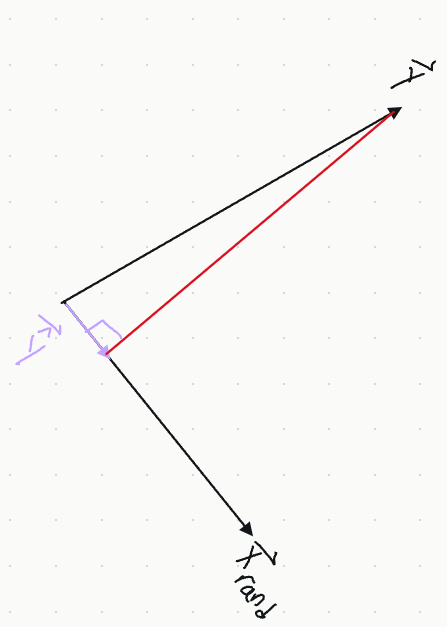
\includegraphics[width=0.3\textwidth]{projecting-onto-xrand}
		\caption{Projectiong $\mathbf{y}$ onto a random vector, resulting
		in chance capitalization}
		\label{fig:chance-capitalization}
	\end{figure}
	This is called \textbf{chance capitalization}. You think it's a fit, but it's not, and you
	are tricking yourself into thinking you got somewhere, but you did not.
	This phenomenon is called \textbf{overfitting}.
	
	Let's continue to add more random vectors to $X$ until it becomes $n\times n$,
	and assume it is full rank. Then $X$ is invertible, and the orthogonal projection
	matrix is now given by
	\begin{align*}
		H
		&= X(X^\top X)^{-1}X^\top\\
		&= \underbrace{XX^{-1}}_{I_n}\underbrace{(X^\top)^{-1}X^\top}_{I_n}\\
		&=I_n
	\end{align*}
	Now if we project $\mathbf{y}$ onto the column space of $X$, we get
	\begin{align*}
		\mathbf{\hat{y}} &=H\mathbf{y}=I_n\mathbf{y}=\mathbf{y}\\
		\mathbf{e}&=\mathbf{y}-\mathbf{\hat{y}}=\mathbf{0}_n
	\end{align*}
	Hence, $SSE=\|\mathbf{e}\|^2=0$, and $R^2=1-\frac{SSE}{SST}=1$; we have a perfect fit.
	This is clearly a problem because we can take a computer, fill our design matrix
	with random junk, and we get a perfect fit. Let's visualize overfitting in the
	case where $p=1$. Then we have $X\in \mathbb{R}^{n\times 2}$:
	\begin{align*}
		X = \begin{bmatrix}
			\mathbf{1}_n \mid \mathbf{x}
		\end{bmatrix}
	\end{align*}
	With high confidence, we can say that our feature $x$ is not the true driver $z$.
	However, if $n=2$ (so we have two data points), we get a perfect fit. A scatterplot
	would look like Figure~\ref{fig:overfitting-n-2-p-1}.
	\begin{figure}
		\centering
		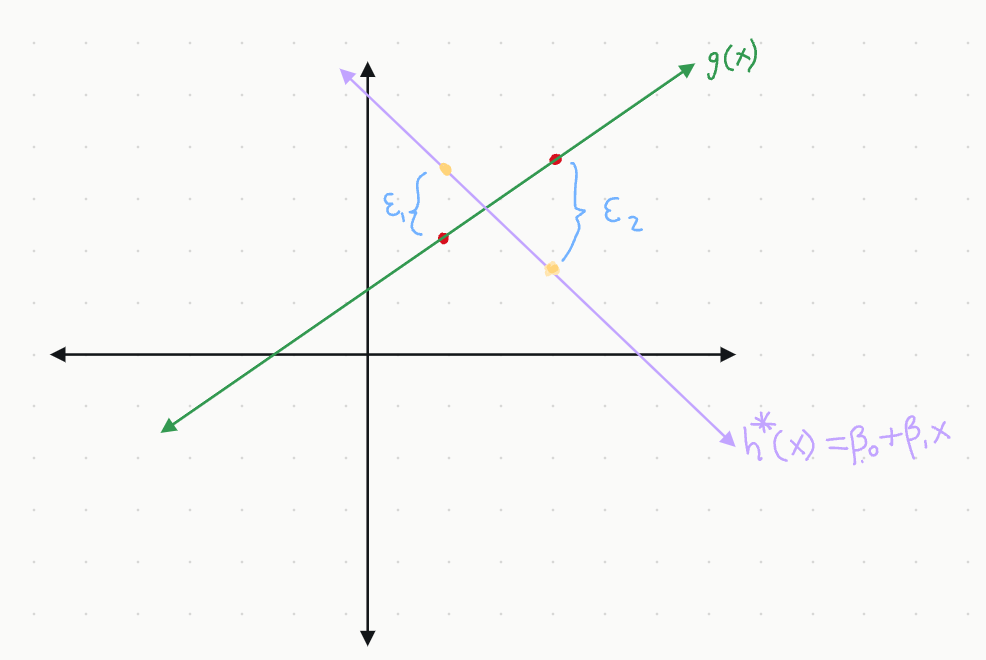
\includegraphics[width=0.5\textwidth]{overfitting-2-points}
		\caption{Overfitting with $n=2$ and $p=1$.}
		\label{fig:overfitting-n-2-p-1}
	\end{figure}
	\section*{Honest Performance Metrics}
	We need honest performance metrics. These should approximate how well we predict
	in the future. Consider that our data set $\mathbf{D}$ is data we have collected
	in the \text{past}. Suppose we were omniscient and had $\mathbb{D}^*$, a data
	set of future data (see Figure~\ref{fig:future-data}).
	\begin{figure}
		\centering
		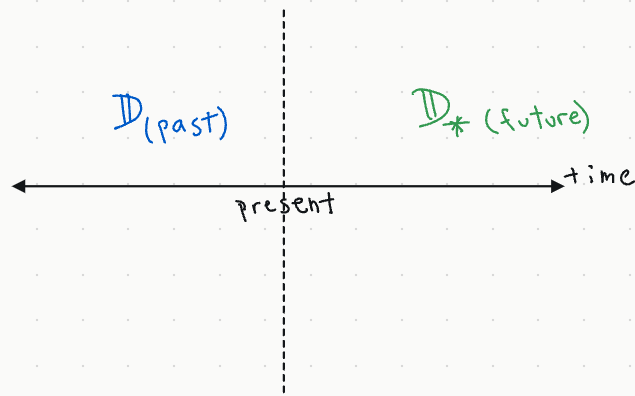
\includegraphics[width=0.4\textwidth]{future-data}
		\caption{Leveraging future data to design honest error metrics.}
		\label{fig:future-data}
	\end{figure}
	We could predict on $X_*$ to get $\mathbf{\hat{y}}_*$, and consider
	$\mathbf{e}_*=\mathbf{y}_*-\mathbf{\hat{y}_*}$, with associated $R_*^2$ and $SSE_*$.
	We will continue this discussion next time.
	\pagebreak
	\printbibliography
\end{document}